\documentclass[a4paper,14pt]{extreport}
\usepackage[left=1.5cm,right=1.5cm,
    top=1.5cm,bottom=2cm,bindingoffset=0cm]{geometry}
\usepackage{scrextend}
\usepackage[T1,T2A]{fontenc}
\usepackage[utf8]{inputenc}
\usepackage[english,russian,ukrainian]{babel}
\usepackage{tabularx}
\usepackage{amssymb}
\usepackage{color}
\usepackage{amsmath}
\usepackage{mathrsfs}
\usepackage{listings}
\usepackage{graphicx}
\graphicspath{ {./images/} }
\usepackage{lipsum}
\usepackage{xcolor}
\usepackage{hyperref}

\usepackage{tcolorbox}
\usepackage{tikz}
\usepackage[framemethod=TikZ]{mdframed}
\usepackage{wrapfig,boxedminipage,lipsum}
\mdfdefinestyle{MyFrame}{%
linecolor=blue,outerlinewidth=2pt,roundcorner=20pt,innertopmargin=\baselineskip,innerbottommargin=\baselineskip,innerrightmargin=20pt,innerleftmargin=20pt,backgroundcolor=gray!50!white}
 \usepackage{csvsimple}
 \usepackage{supertabular}
\usepackage{pdflscape}
\usepackage{fancyvrb}
%\usepackage{comment}
\definecolor{ggreen}{rgb}{0.,1,0}
\definecolor{rred}{rgb}{1,0.1,0.1}
\usepackage{array,tabularx}
\usepackage{colortbl}

\usepackage{varwidth}
\tcbuselibrary{skins}
\usepackage{fancybox}




\usepackage{float}
\usepackage{wrapfig}
\usepackage{framed}





\begin{document}
\pagecolor{white}
\begin{titlepage}
  \begin{center}
    \large
    Національний технічний університет України \\ "Київський політехнічний інститут імені Ігоря Сікорського"


    Факультет Електроніки

    Кафедра мікроелектроніки
    \vfill

    \textsc{ЗВІТ}\\

    {\Large Про виконання лабораторної роботи №1\\
      з дисципліни: «Твердотільна електроніки-1»\\[1cm]

    ДОСЛІДЖЕННЯ ВИПРЯМЛЯЮЧИХ НАПІВПРОВІДНИКОВИХ ДІОДІВ\\

    }
  \bigskip
\end{center}
\vfill

\newlength{\ML}
\settowidth{\ML}{«\underline{\hspace{0.4cm}}» \underline{\hspace{2cm}}}
\hfill
\begin{minipage}{1\textwidth}
Виконавець:\\
Студент 3-го курсу \hspace{4cm} $\underset{\text{(підпис)}}{\underline{\hspace{0.2\textwidth}}}$  \hspace{1cm}А.\,Р.~Півчук\\
\vspace{1cm}

Перевірив: \hspace{6.1cm} $\underset{\text{(підпис)}}{\underline{\hspace{0.2\textwidth}}}$  \hspace{1cm}Л.\,М.~Королевич\\

\end{minipage}

\vfill

\begin{center}
2020
\end{center}
\end{titlepage}
%---------------------------------------------------------------------------------------------------------------------------------------------------------------------------------



\begin{center}1. МЕТА РОБОТИ\\ \end{center}

Теоретичне вивчення і практичне дослідження випрямляючих діодів; визначення фізичних та основних технічних параметрів германійових та кремнійових діодів із їх вольт-амперних характеристик.\\

\begin{center}2. ЗАВДАННЯ\\ \end{center}

1. Вивчити структуру параметрів (паспортних даних) досліджуваного підкласу діодів.
Ознайомитися із вимірювальним стендом та використовуваними приладами.\par
2. Зібрати схему для дослідження вольт-амперної характеристики випрямляючих діодів.\par
3. Виміряти вольт-амперні характеристики германійового та кремнійового діодів при
кімнатній температурі. Результати вимірювань записати в таблиці.\par
4. *Провести температурні дослідження ВАХ германійового та кремнійового діодів при
температурі $+70^\circ$ С (для прямої та зворотньої полярності напруги).\par
5. Побудувати графіки вольт-амперних характеристик діодів.\par
6. Графічно визначити дифузійний потенціал $\phi_0$ , опір бази $r_b$ та струм виродження $I_\text{вир}$ для
кожного з діодів. Оцінити тепловий струм германійового діода.\par
7. За побудованими графіками характеристик визначити основні параметри діодів.\par
8. **Побудувати графіки залежностей статичного та динамічного опорів діодів від
прикладеної напруги (або вирахувати статичний та диференційний опори посередині прямої та
зворотньої гілок ВАХ кожного діоду і співставити їх між собою).\par
9. Провести аналіз результатів досліджень, і зробити висновки з виконаної роботи.
\newpage
%---------------------------------------------------------------------------------------------------------------------------------------------------------------------------------



\begin{center}
\begin{figure}[h]
\center{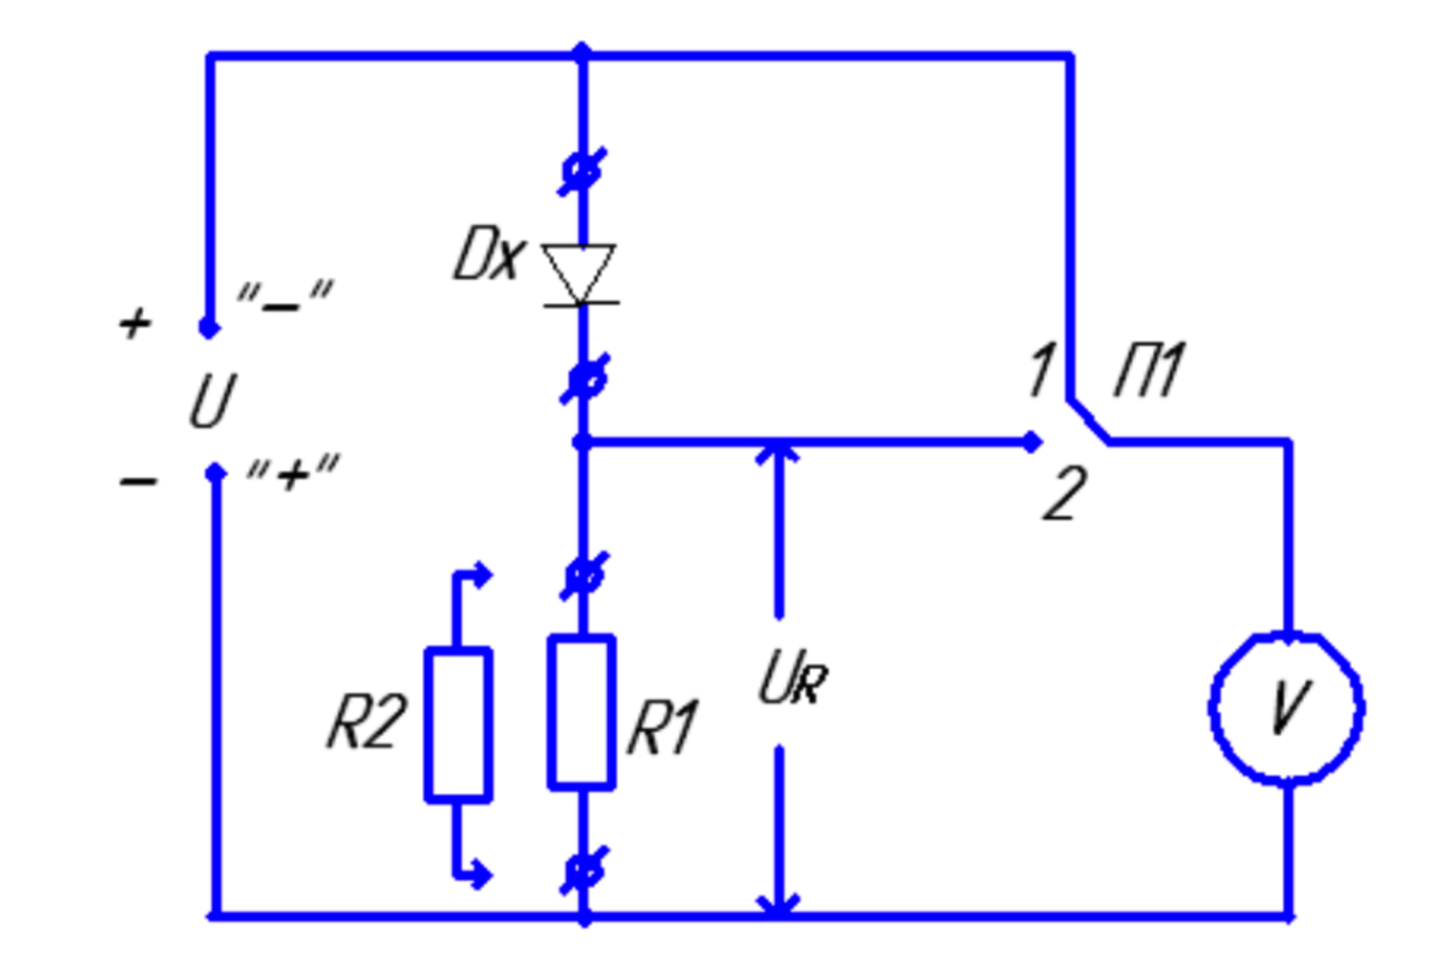
\includegraphics[height=10 cm, width=15 cm]{1.1.png}}
\caption[wec]{ \centering{Схема для вимірювання ВАХ діода. При знятті зворотньої гілки ВАХ змінюється
полярність джерела живлення та номінал резистора R (величина резистора для прямої гілки $R _1$ = 5 кОм; для зворотньої $R _2$  = 100 кОм, або 1 МОм).}}
\label{ris:image}
\end{figure}
\end{center}








%1---------------------------------------------------------------------------------------------------------------------------------------------------------------------------------
\clearpage
\newpage
\begin{center}3.РЕЗУЛЬТАТИ ВИМІРЮВАНЬ\\ \end{center}
\begin{center}3.1.Обрахунки значень\\ \end{center}
Всі значення та їх похибкибки обраховувались за наступними формулами:\\
Значення спаду напруги на діоді:
\begin{equation}
U_D = U-U_R
\end{equation}

Значення струму через діод:
\begin{equation}
I_D = \dfrac{U_R}R
\end{equation}

Значення опору бази:
\begin{equation}
r_b = \dfrac{U_{\text{пр}} - \varphi_0}{I_{\text{пр}}}
\end{equation}

Значення струму виродження:
\begin{equation}
I_{\text{вир}} = \dfrac{\varphi_T}{r_b}
\end{equation}

Та їх похибки:
\begin{equation}
\triangle U_D = \sqrt{\triangle U^2 +\triangle U_R^2 }
\label{eq:ref}
\end{equation}

\begin{equation}
\triangle I_D = \dfrac 1{R^2} \cdot \sqrt {(R\triangle U_R)^2 + (U_R\triangle R)^2}
\label{eq:ref}
\end{equation}

\clearpage
\newpage
\begin{center}3.2.Представлення значень у вигляді таблиць\\ \end{center}
\begin{center}
\begin{figure}[h!]
\center{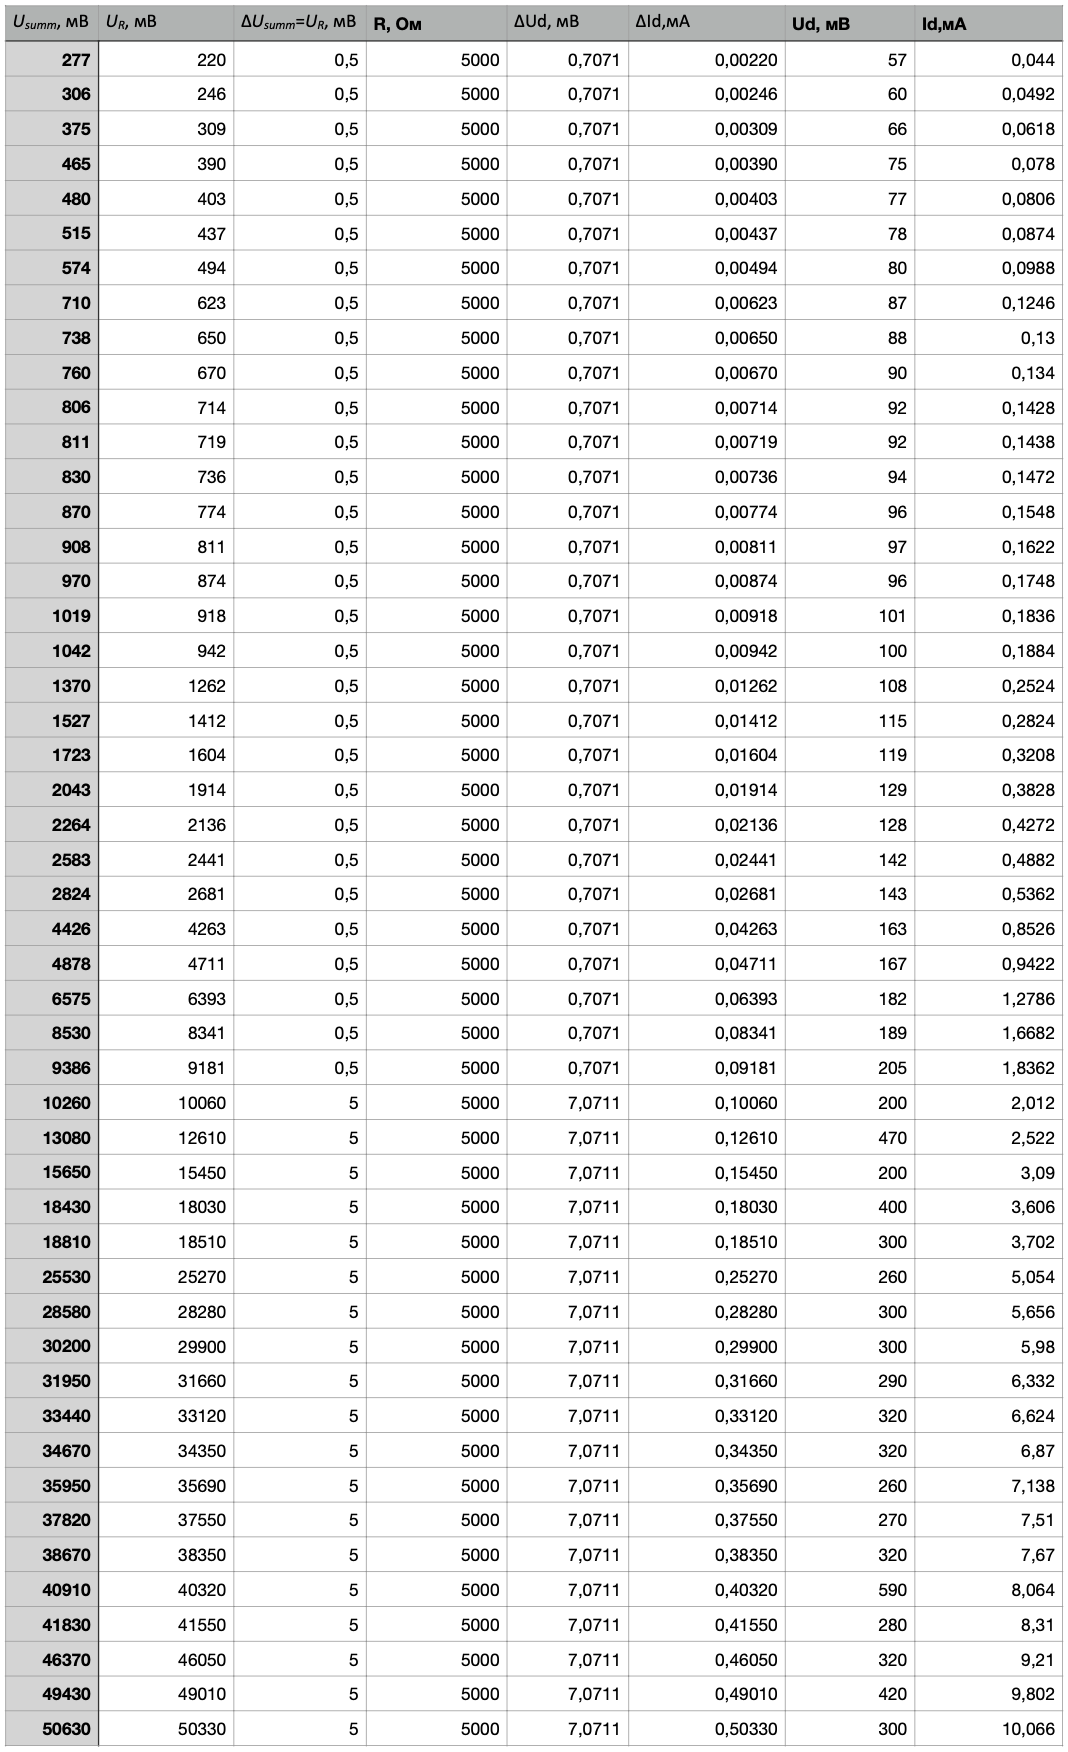
\includegraphics[scale = 0.75]{1.png}}\\
\centering{Табл. 1: ВАХ дiода D1 за прямого змiщення.}
\label{ris:image}
\end{figure}
\end{center}




%2---------------------------------------------------------------------------------------------------------------------------------------------------------------------------------
\clearpage
\newpage
\begin{center}
\begin{figure}[h]
\center{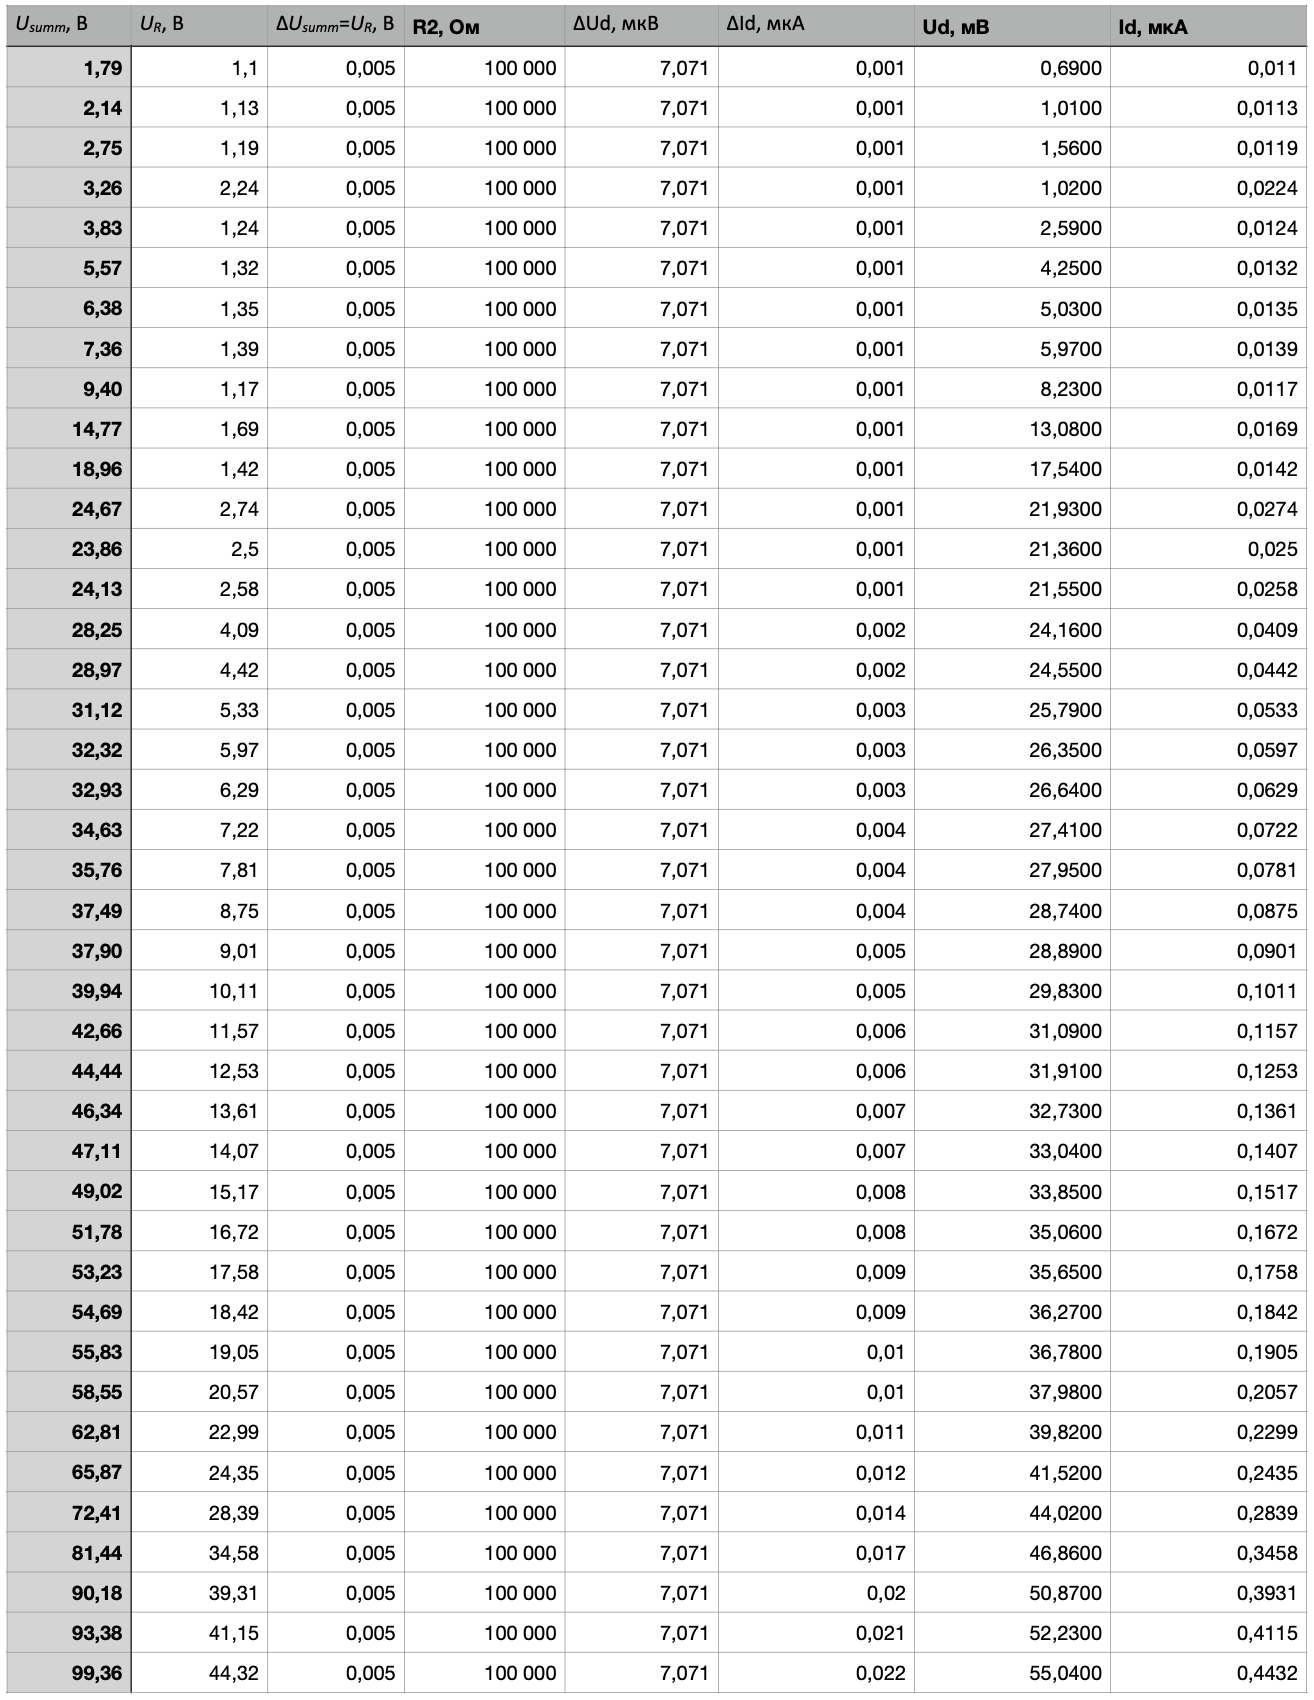
\includegraphics[height=22 cm, width=17 cm]{2.png}}
 \centering{Табл. 2: ВАХ дiода D1 за зворотного змiщення.}
\label{ris:image}
\end{figure}
\end{center}


%3---------------------------------------------------------------------------------------------------------------------------------------------------------------------------------
\clearpage
\newpage
\begin{center}
\begin{figure}[h]
\center{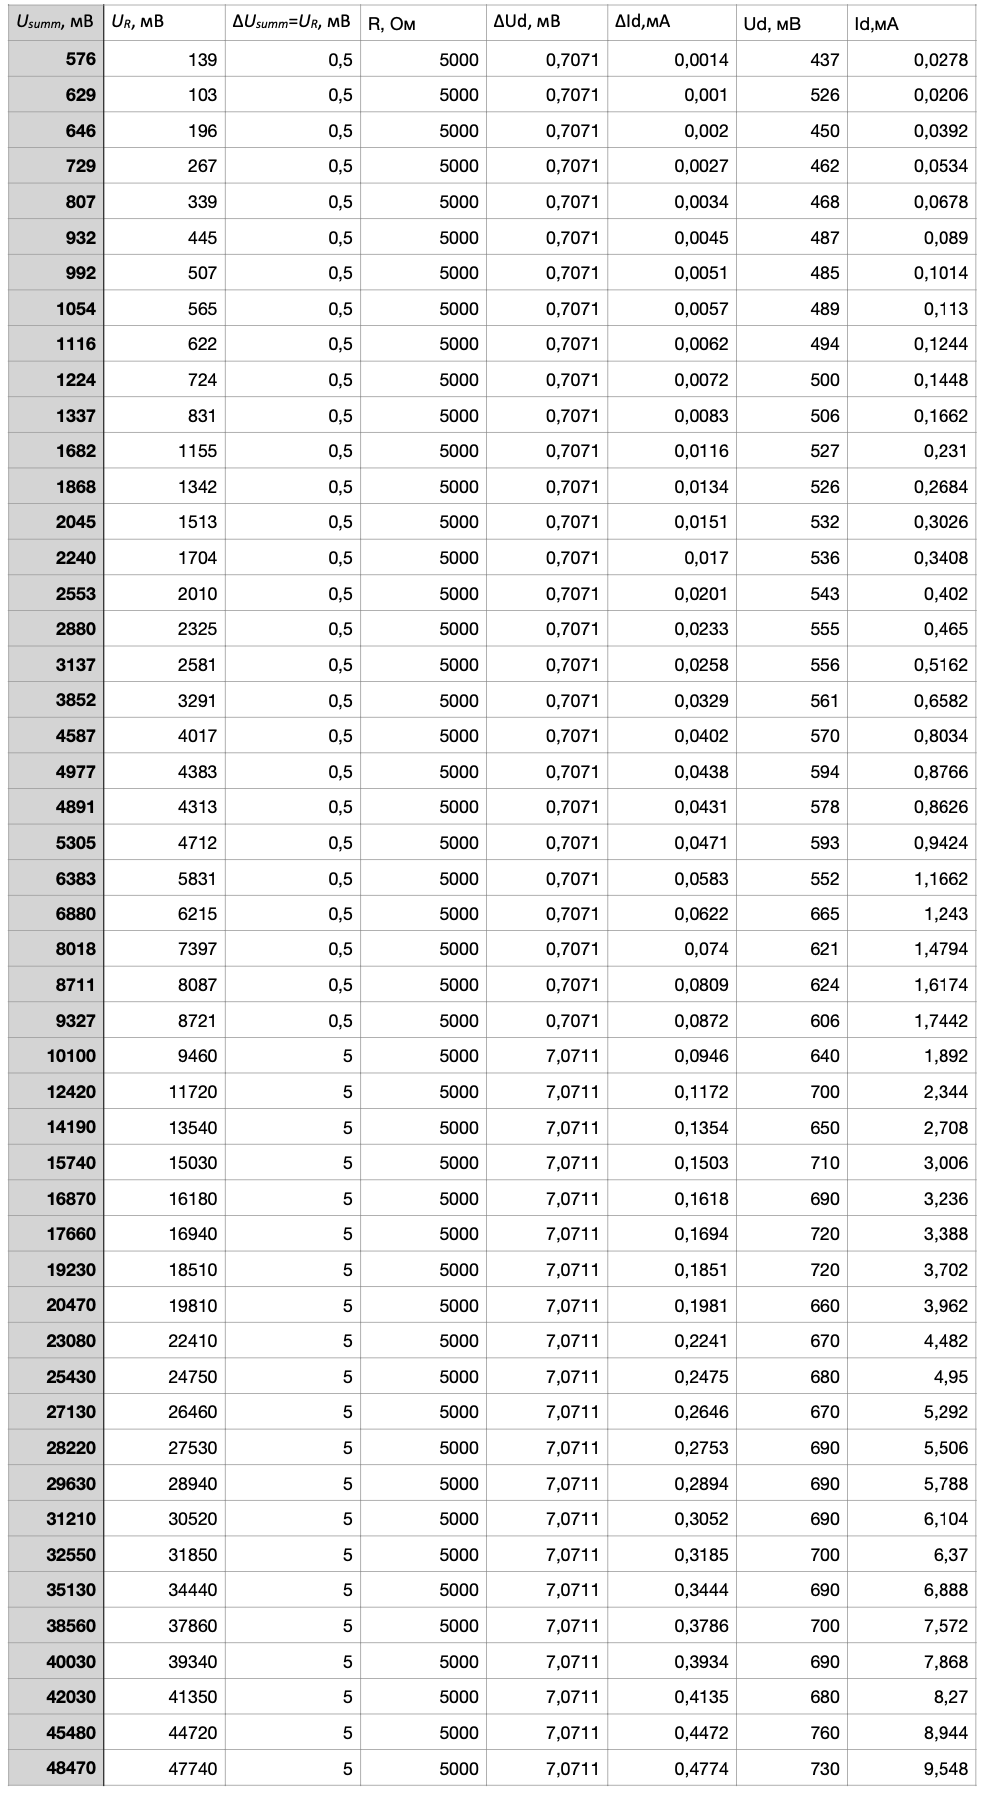
\includegraphics[height=26 cm, width=17 cm]{3.png}}
\centering{Табл. 3: ВАХ дiода D2 за прямого змiщення.}
\label{ris:image}
\end{figure}
\end{center}


%4---------------------------------------------------------------------------------------------------------------------------------------------------------------------------------
\clearpage
\newpage
\begin{center}
\begin{figure}[h]
\center{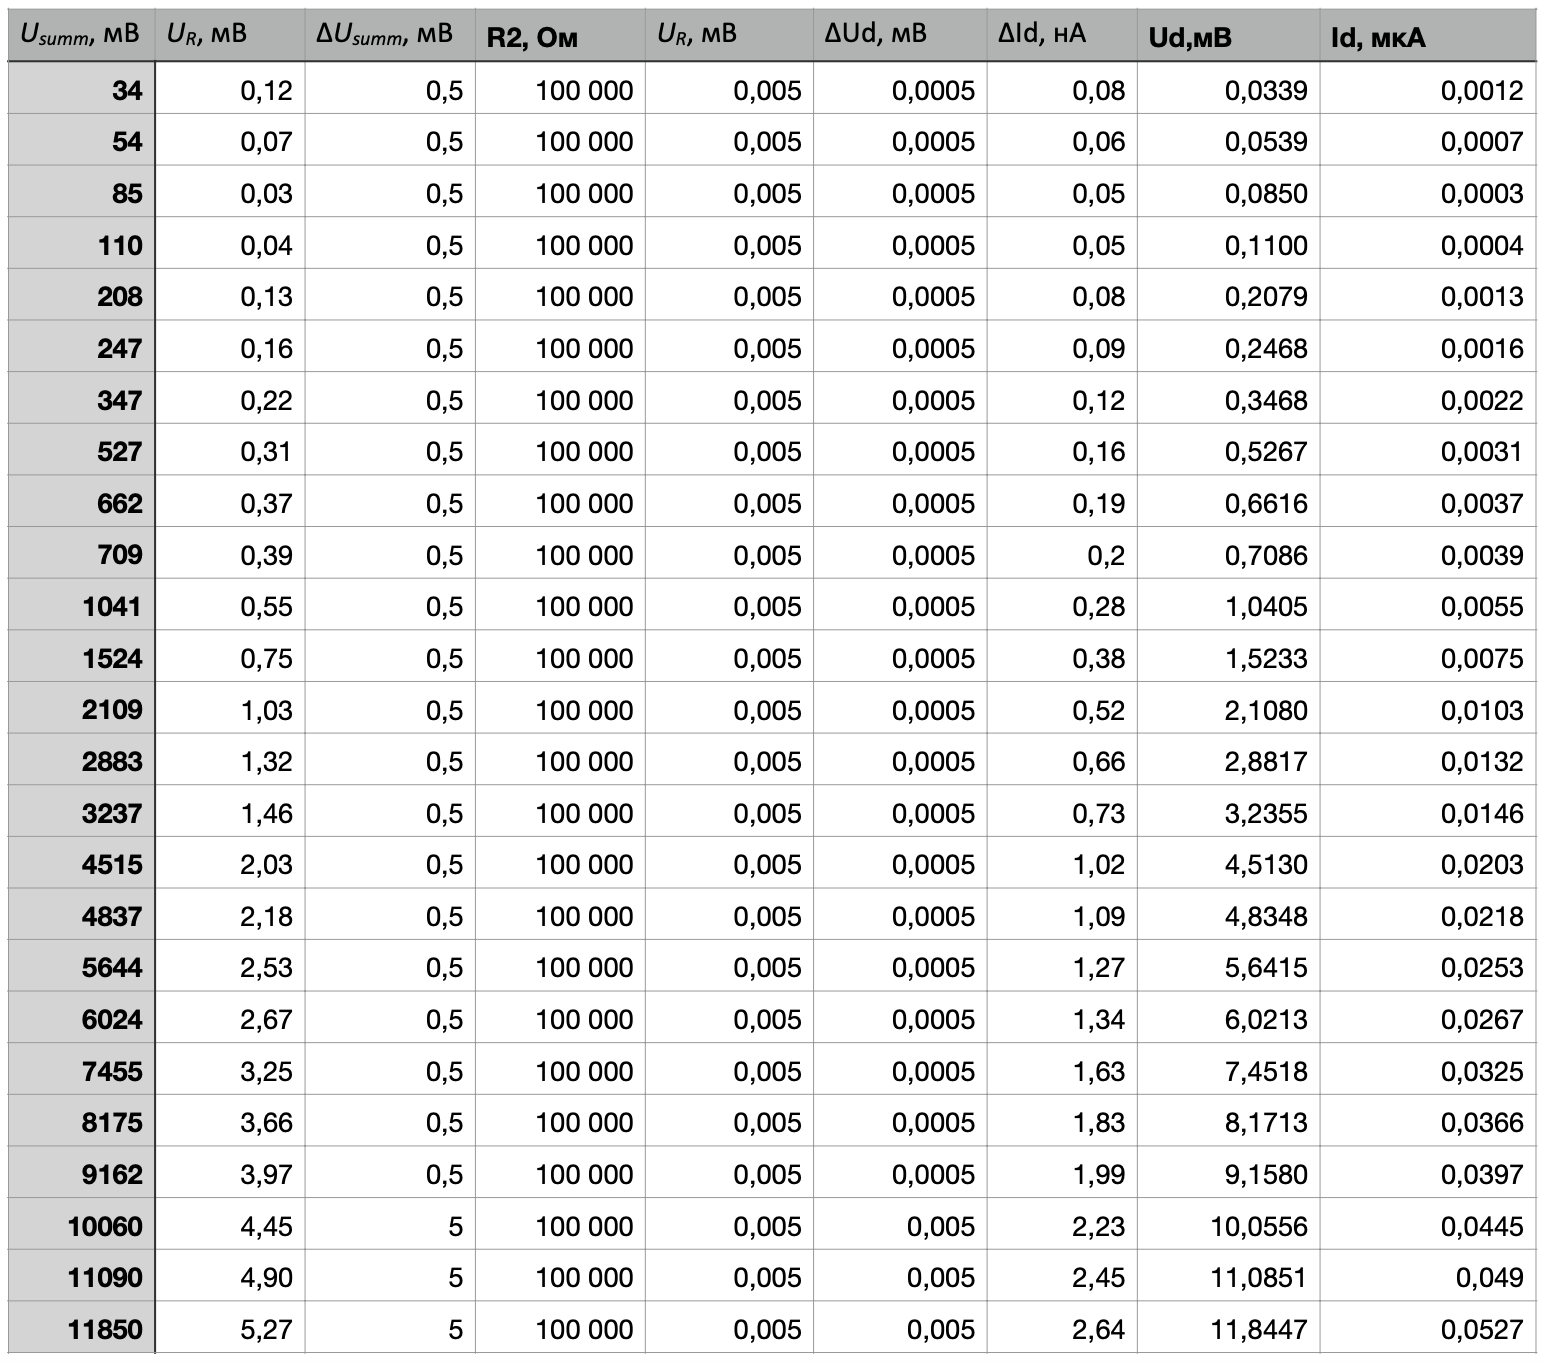
\includegraphics[height=15 cm, width=17 cm]{4.png}}
\centering{Табл. 4: ВАХ дiода D2 за зворотного змiщення.}
\label{ris:image}
\end{figure}
\end{center}
\vspace{1cm}

\clearpage
\newpage
\vspace{1cm}





%ГРАФІКИ---------------------------------------------------------------------------------------------------------------------------------------------------------------------------------
\newpage
\begin{center}3.1. ГРАФІКИ\\ \end{center}



\begin{figure}[h]
\center{\includegraphics[width=1\linewidth]{d1.pdf}}
\caption{ВАХ дiода D1 за прямого змiщення.}
\label{ris:image04}
\end{figure}


\begin{figure}[h]
\center{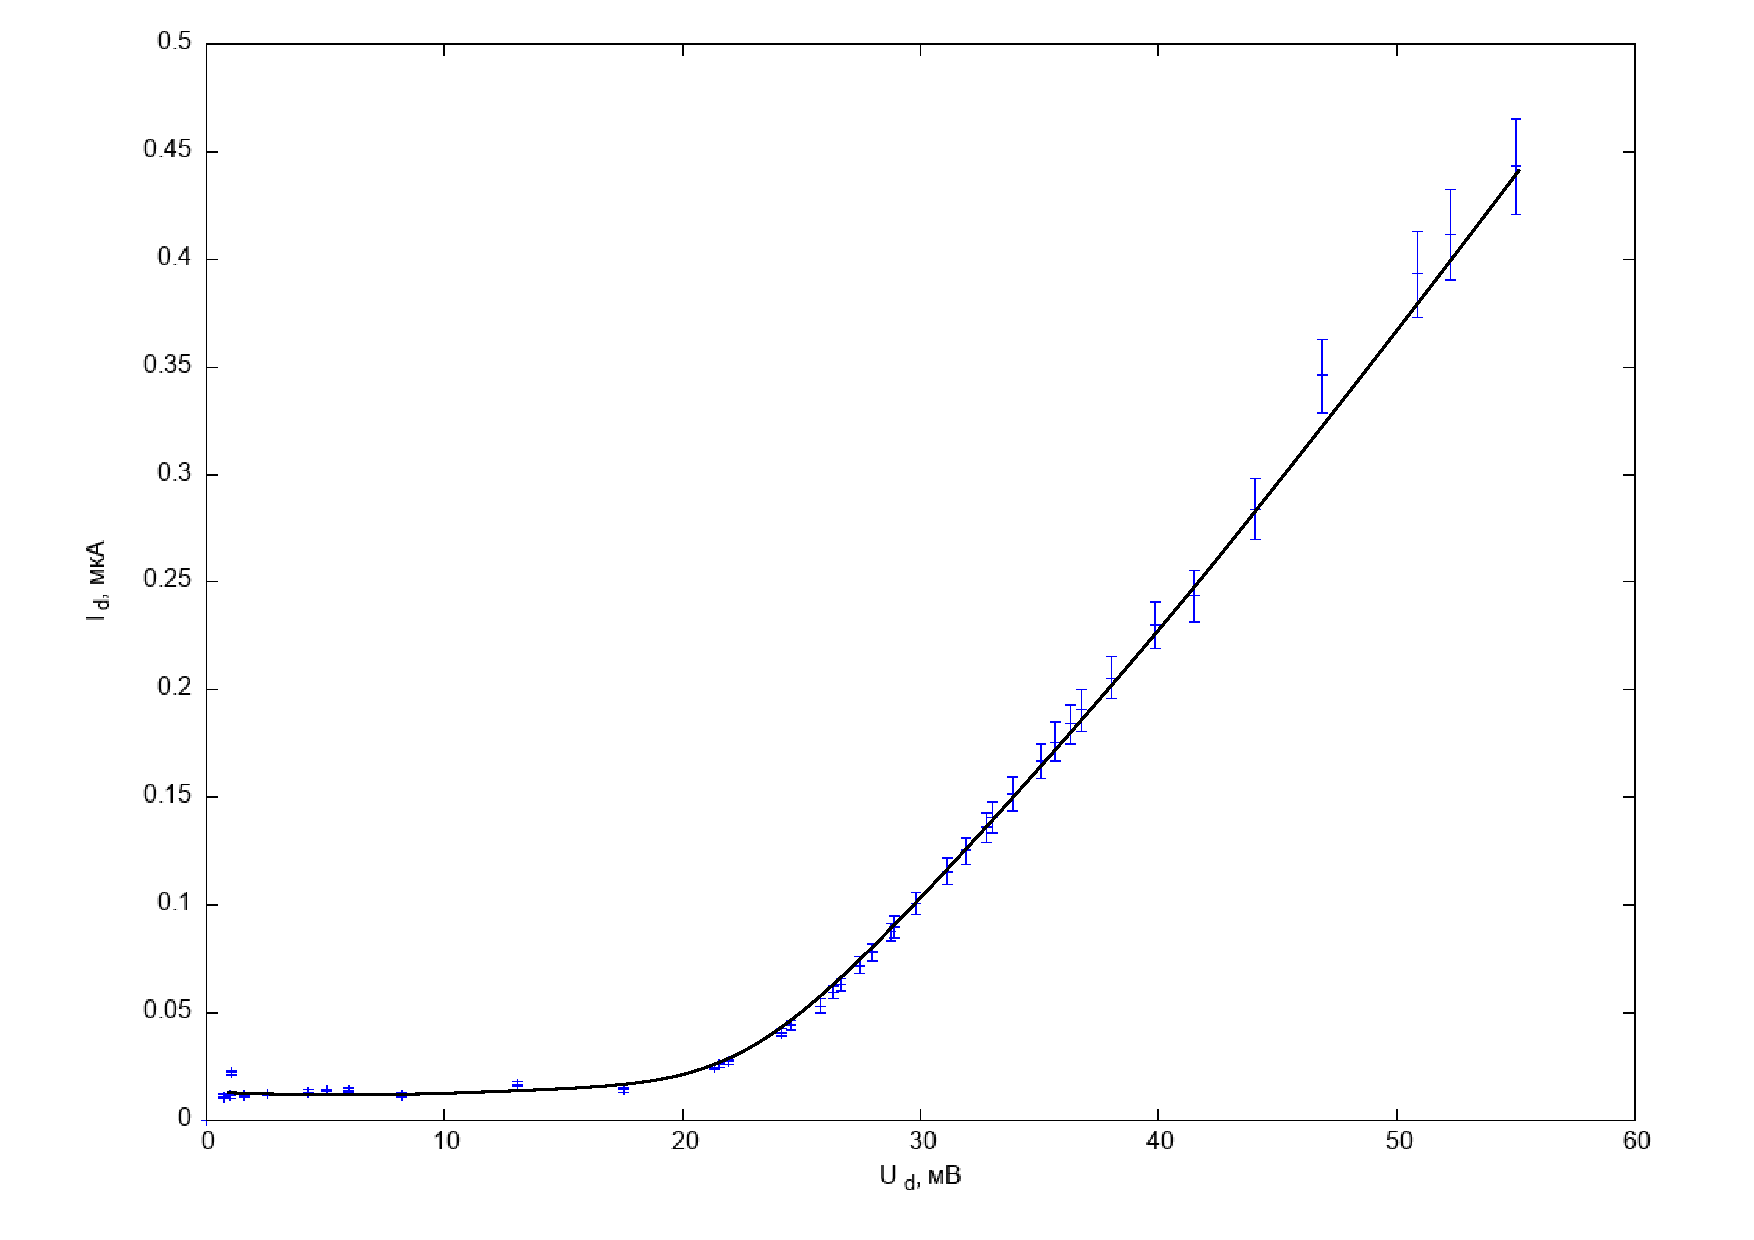
\includegraphics[width=1\linewidth]{d1r.pdf}}
\caption{ВАХ дiода D1 за зворотного змiщення.}
\label{ris:image4}
\end{figure}


\begin{figure}[h!]
\center{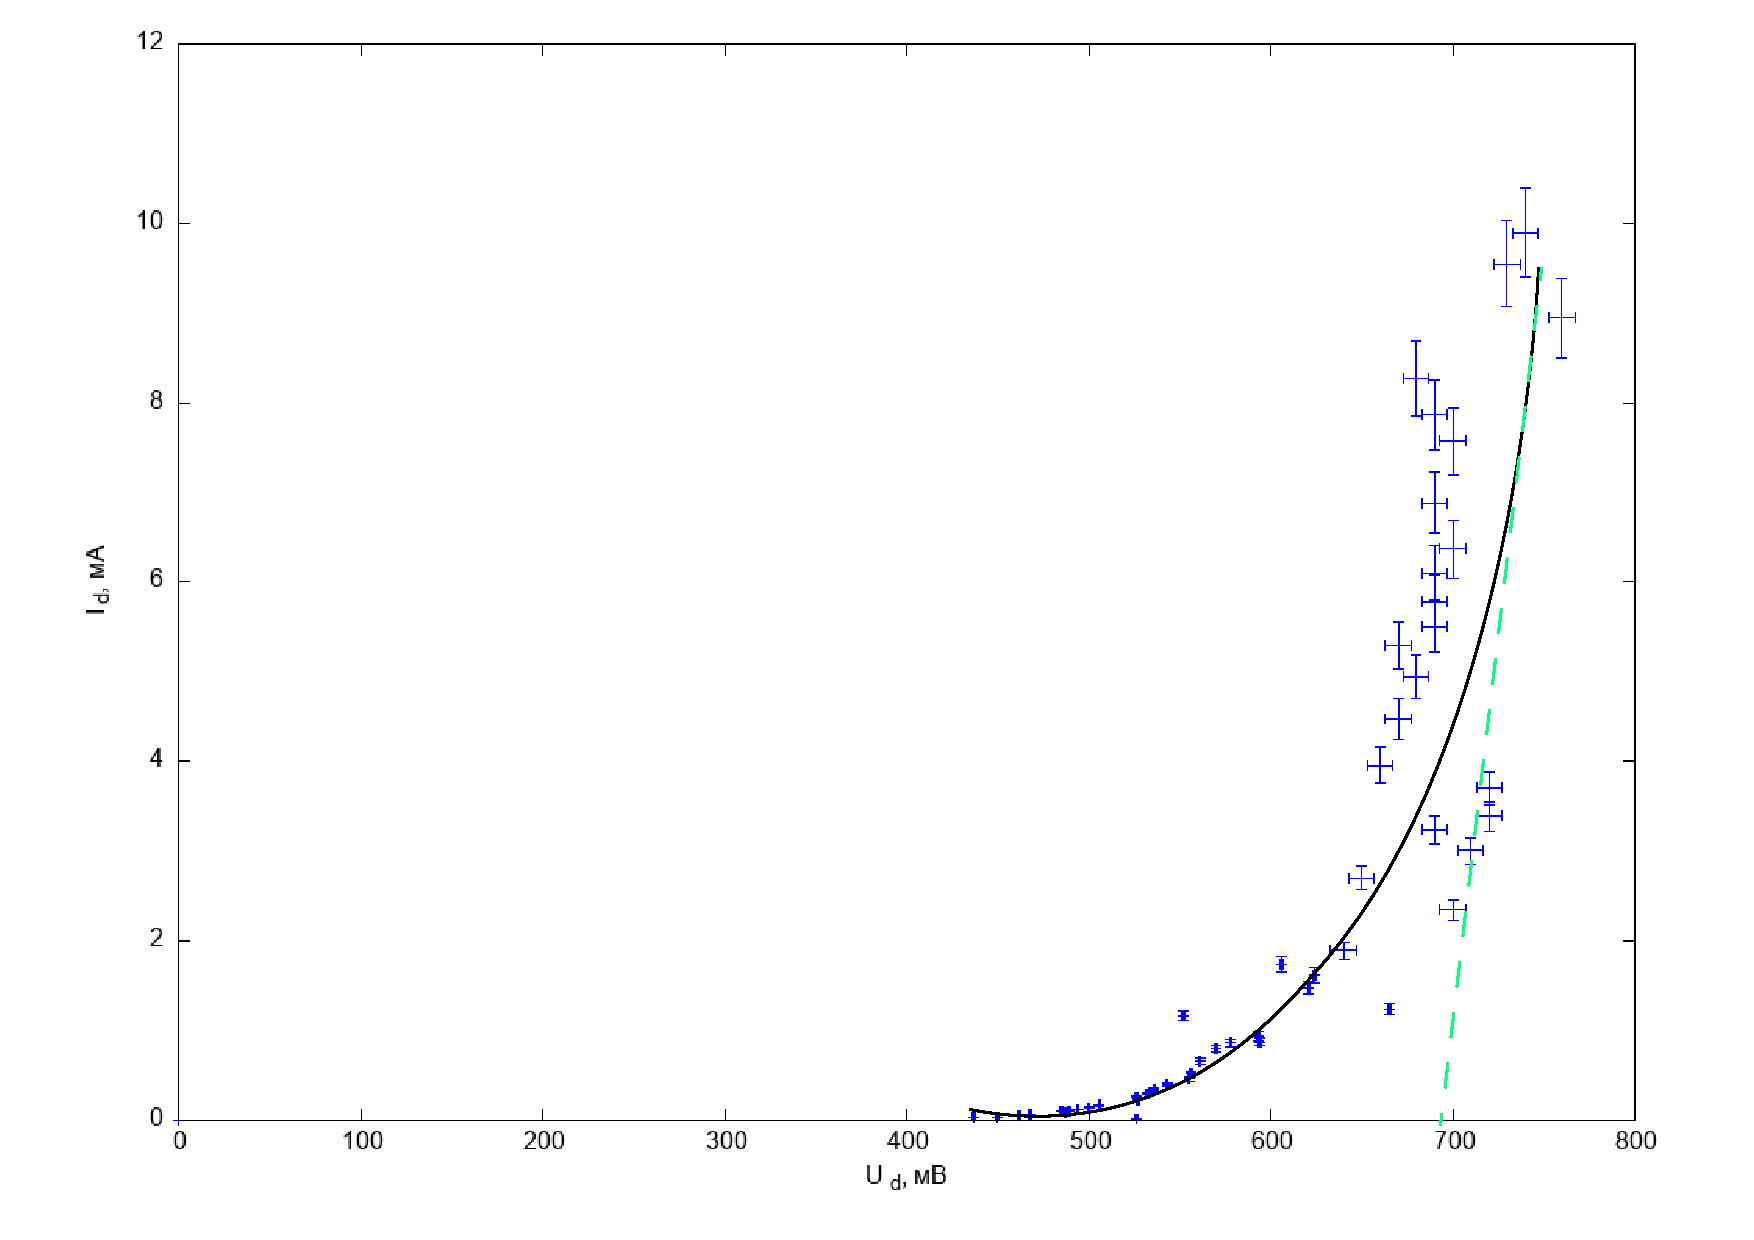
\includegraphics[width=1\linewidth]{d2.pdf}}
\caption{ВАХ дiода D2 за прямого змiщення.}
\label{ris:image05}
\end{figure}


\begin{figure}[h]
\center{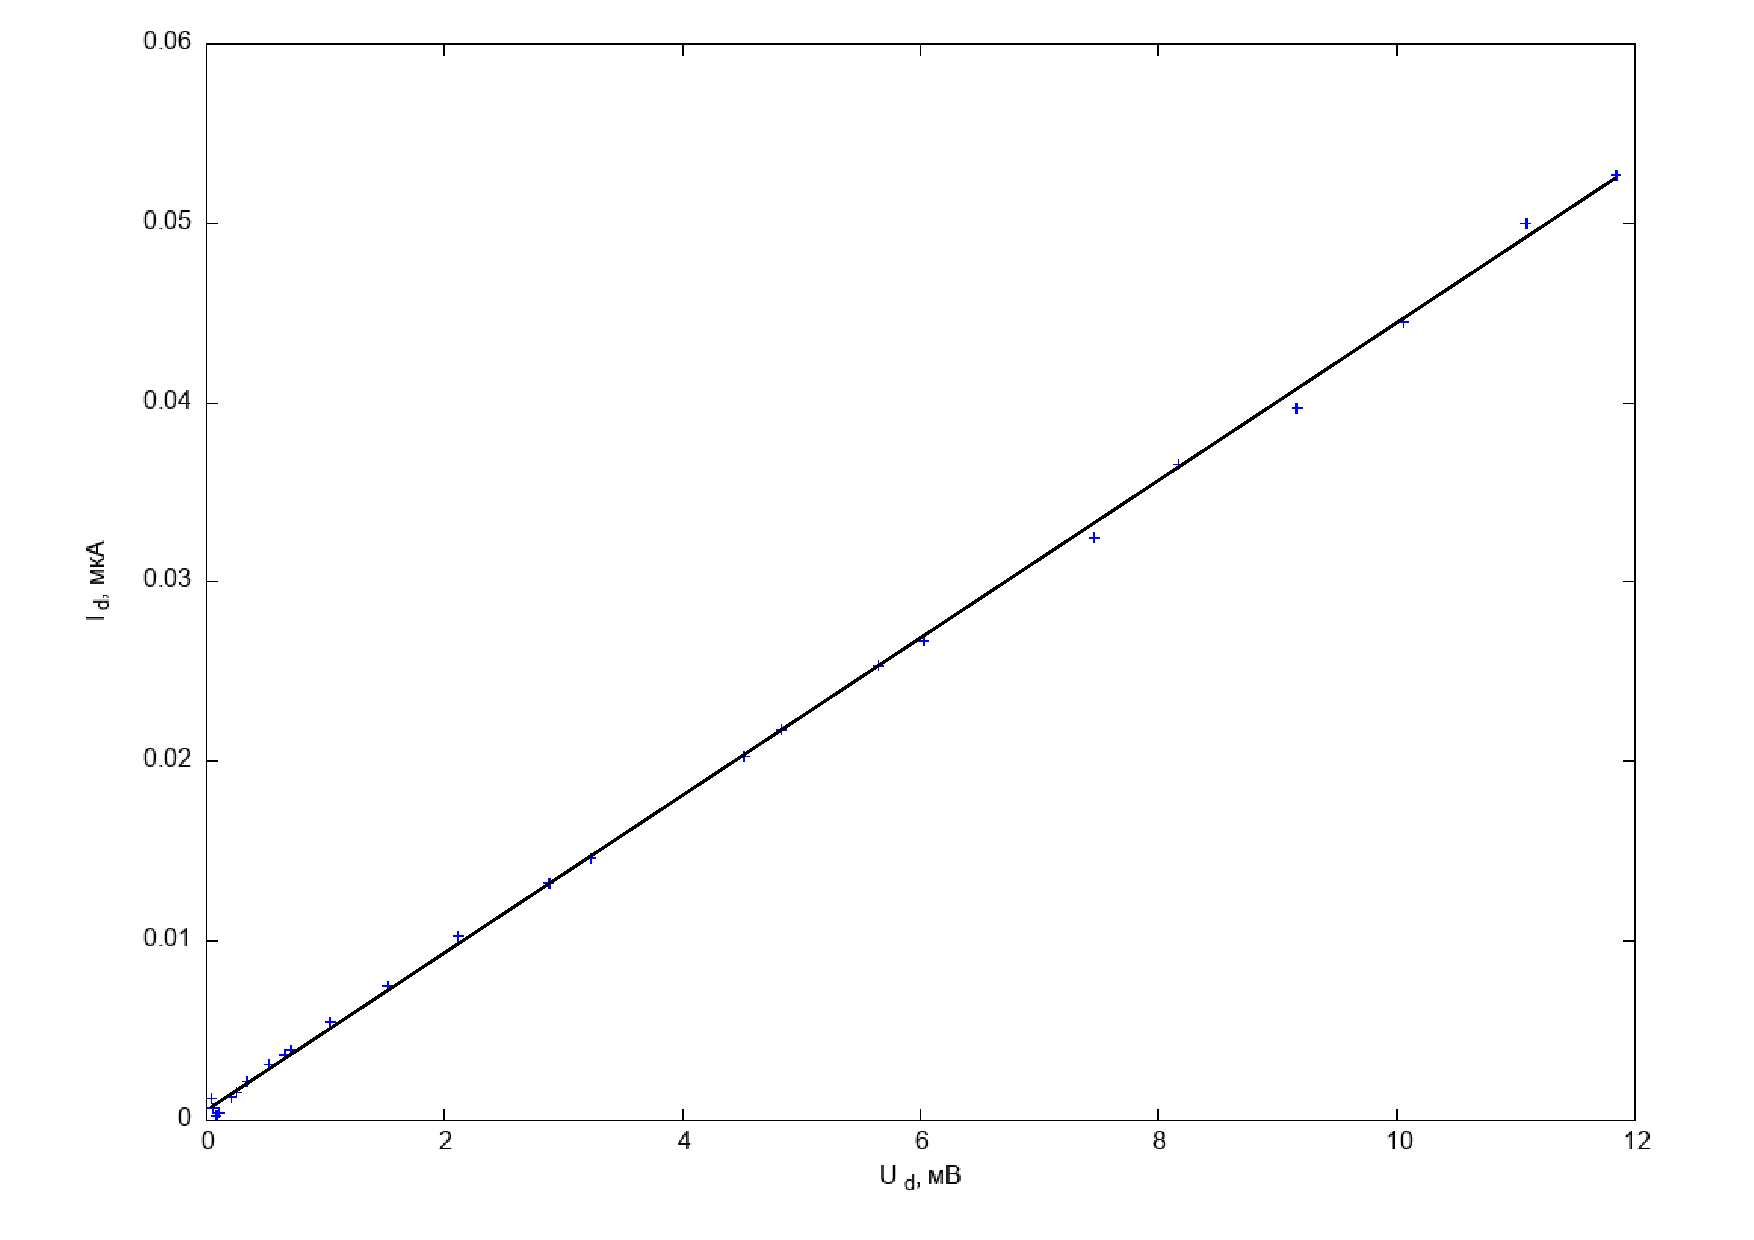
\includegraphics[width=1\linewidth]{d2r.pdf}}
\caption{ВАХ дiода D2 за зворотного змiщення.}
\label{ris:image4}
\end{figure}
%---------------------------------------------------------------------------------------------------------------------------------------------------------------------------------

\clearpage
\newpage
\begin{center}3.2. Розрахунок $r_b$ та $I_{\text{вир}}$ для двох діодів\\ \end{center}

Використовуючи Рис. (2)  опір бази $r_b$ D1: для цього з точки T опускаємо перпендикуляр на обидві осі, потім визначаємо значення в точці їх перетину $I_{\text{пр}} = $ 0.008 А і $U_{\text{пр}} = $ 0,3 В. Наступним кроком знайдемо дифузійний потенціал який знаходиться в точці перетину дотичної проведеної до точки Т і вісі напруг. Зробивши це отримаємо $\varphi_0 = $ 0.255 В.

\begin{equation}
r_b = \dfrac{U_{\text{пр}} - \varphi_0}{I_{\text{пр}}} = 5.624 \text{ Ом}
\label{eq:ref}
\end{equation}

Тепер можемо знайти $I_{\text{вир}}$:
\begin{equation}
I_{\text{вир}} = \dfrac{\varphi_T}{r_b} = 0.0046 \text{ A}
\label{eq:ref}
\end{equation}

Аналогічно для діода D2:
\begin{center}
$I_{\text{пр}} = 0.007$ А\\
\vspace{0.3cm}
$U_{\text{пр}} = 0.73$ В\\
\vspace{0.3cm}
$\varphi_0 = 0.69$ В\\
\vspace{0.3cm}
$r_b =  5.7142 $Ом\\
\vspace{0.3cm}
$I_{\text{вир}} =0.0045$ А\\
\vspace{0.3cm}
\label{eq:ref}
\end{center}


%---------------------------------------------------------------------------------------------------------------------------------------------------------------------------------
\clearpage
\newpage
\begin{center}4. АНАЛІЗ РЕЗУЛЬТАТІВ ДОСЛІДЖЕНЬ ТА ВИСНОВКИ З ВИКОНАНОЇ РОБОТИ\\ \end{center}

В результаті виконання даної лабораторної роботи було досліджено випрямляючі діоди та побудовно графіки ВАХ германієвого та кремнієвого діодів. Також виходячи з вольт-фмперної характеристики діода D1 можна сказати що це германієвий діод, оскільки спад напруги в прямому напрямі на германієвих діодах не перевищує 0,5 В, а що стосується діода під назвою D2 то як видно з його ВАХ за прямого зміщення то це кремнієвий діод, оскільки прямий спад напруги у кремнієвих діодах більший, ніж у германієвих, і досягає 1,5 В.
















\end{document}
